In this section, we provide a brief overview of particle dark matter candidates.

{\it Weakly-Interacting Massive Particles (WIMPs)}: In the WIMP paradigm, the dark matter candidate has a mass of $\roughly 100 \GeV$ and interacts with Standard Model particles via weak-scale interactions. In the early universe, the WIMP can be produced in the thermal bath of Standard Model particles, and its abundance is set by the so-called “freeze-out” process, i.e., when the annihilation rate between two WIMPs to Standard Model particles drops below the Hubble expansion rate, the co-moving number density of WIMPs remains nearly constant over the evolution. It turns out the weak-scale interactions lead to a WIMP relic abundance, consistent with the observed dark matter abundance. Over the past thirty years, the WIMP paradigm has motivated a number of searches in terrestrial experiments, including dark matter direct and indirect experiments, as well as collider experiments. The WIMP is a typical CDM candidate, and for a WIMP mass of $\roughly 100 \GeV$ the minimal halo mass is $\roughly 1 M_\Earth$.

\begin{comment}
\ADW{I do not see how LSST provides input on this model of dark matter}
{\it Asymmetric dark matter}: The asymmetry between baryons and anti-baryons is well-documented in the visible sector, and can be trivially generalized to the dark matter sector. In this theory, the dark matter abundance is set by some primordial asymmetry in the early universe and further annihilation deplete the asymmetry component and only dark matter presents in the present universe. An attractive feature of this theory is that both dark matter and baryonic matter can be co-generated in the early universe and it explains the observational coincidence that the dark matter abundance is 5 times higher than the baryon abundance. For asymmetric dark matter, the typical dark matter mass is close to $5~{\rm GeV}$, five times the proton mass. For asymmetric dark matter, indirect detection signals from dark matter annihilation are typically absent, while direct and collider signals would be similar as in the WIMP case.
\end{comment}

{\it Hidden sector dark matter}: given the fact that we have not seen any signals from the terrestrial searches, there has been growing interest in the hidden sector dark matter theory. It assumes the dark matter is just one component of a more complex dark sector that may compose of multiple particle species. In the early universe, these hidden particles can be produced through inflaton decays, similar to the standard model particles. The dark matter abundance can be set by the freeze-out or asymmetric mechanisms. In some realizations, one can still preserve the virtue of the WIMP miracle. The hidden sector could also couple to the standard model sector through some portals, e.g., kinetic mixing, Higgs and neutrino mixings. And these mixing portals may lead to indirect and direct detection signals. In addition, if these portal terms present, the dark matter abundance can be produced through the freeze-in mechanisms, or even the hidden sector can be thermalized with the standard model sector. However, since the correlation between the dark matter abundance and the mixing parameter is loosened, compared to the WIMP case, it is possible to have the correct relic abundance while being consistent with the terrestrial constraints. In the hidden dark matter theory, model constraints on the dark matter mass and interactions are typically weak, which allows large model parameters subject to astrophysical probes. Possibilities are richer compared to the WIMP case.
\ADW{I think this needs to be connected back to LSST. For example, coupling between dark matter and dark radiation can be constrained via ETHOS-like frameworks.}

{\it Self-interacting dark matter (SIDM)}: SIDM assumes that dark matter has strong self-interactions analogous to the nuclear interactions. Dark matter self-interactions thermalize the inner regions of dark matter halos, where galaxies sit, and tie the dark matter and luminous matter distributions. For low-surface brightness galaxies, SIDM thermalization leads to a cored inner density profile, in contrast to the cupsy profiles predicted in CDM. While for high-surface brightness galaxies, thermalization leads to a small core and more concentrated SIDM distribution because of the presence of the baryonic potential. It has been shown that SIDM can explain both the diversity and uniformity of galaxy rotation curves for the self-scattering cross section per unit mass $\sigma/m>\mathcal{O}(1\cmg)$ on galactic scales. There are constraints on the self-scattering cross section, such as merging clusters and halo shapes of elliptical galaxies. Notably, observations from well-relaxed galaxy clusters show $\sigma/m\sim0.1\cmg$ to be consistent with their inferred core sizes. 

SIDM could also have a measureable impact the matter power spectrum. In SIDM models where dark matter particle couples to a massless particle in the early universe through a light mediator, the tight coupling between dark matter and dark radiation can lead to dark acoustic oscillations, resulting a suppressed and oscillatory power spectrum. The minimal halo masses can be around $10^5\textup{--}10^8M_\odot$, depending on the model halo parameters.      

{\it Warm dark matter (WDM)}: the warm dark matter candidate a long free-streaming length, resulting in a cutoff on halo abundance for low-mass halos. In the warm dark matter theory, dark matter typically has a light mass around few keV such that it decouples from the thermal bath late and lead to a long free-streaming length. Typical warm dark matter candidates include sterile neutrinos. In warm dark matter, structure formation of the universe occurs bottom-up above the free-streaming scale, while top-down for scale below the free-streaming scale. The measurements of the Lyman-alpha forest put lower bounds on the mass of warm dark matter produced thermally 3.5 (5.3) keV [], corresponding to the minimal halo mass $10^9\textup{--}10^10M_\odot$.

In the standard thermal dark matter paradigm, primordial inhomogeneities in the matter density field are washed out by collisional damping and free streaming of particle dark matter \citep{Hofmann:2001,Green:2003un, Bertschinger:2006nq, Loeb:2005pm}.  For a canonical 100-GeV thermal relic dark matter particle, these processes erase cosmological perturbations with $M \leq 10^{-6} \Msun$ \citep[i.e., Earth mass][]{Green:2003un}. Lighter particles continue to free stream at lower temperatures (later times), thus suppressing the formation of structure at higher mass scales.

Free-streaming also sets the low-mass end of clustering in sterile neutrino dark matter models, which decouple from the primordial plasma while they are relativistic. In this case, the free-streaming scale can be approximated by the (comoving) size of the horizon when the sterile neutrinos become nonrelativistic. The comoving horizon size at $z = 10^7$ corresponds to $m = 2.5 \keV$, and is approximately $50 \kpc$, which is significantly smaller than the scale derived above for $\Lstar$ galaxies (Adhikari et al. 2017). 

Astrophysical constraints are generally placed on warm dark matter by observing the smallest gravitationally bound dark matter halos.  The half-mode scale, the scale at which the dark matter transfer function is reduced by half, represents a characteristic halo mass scale where observations can be performed. 
The half-mode halo mass, $M_{hm}$, is related to the WDM particle mass, $m_{\rm WDM}$, by \citep{Bullock:2017xww}
\begin{equation}
    M_{\rm hm} = 5.5 \times 10^{10} \big ( \frac{m_{\rm WDM}}{1 {\rm keV}} \big)^{-3.33} {\rm M_\odot}.
\end{equation}
Thus, an observed suppression in the abundance of dark matter halos smaller than a given scale, $M_{hm}$, could signify the existence of a thermal dark matter particle with mass,
\begin{equation}
    m_{\rm WDM} =  3.33 \big ( \frac{M_{hm}}{10^{9} {\rm M_\odot}} \big)^{-0.3} {\rm keV}
\end{equation}

\begin{figure}
\centering
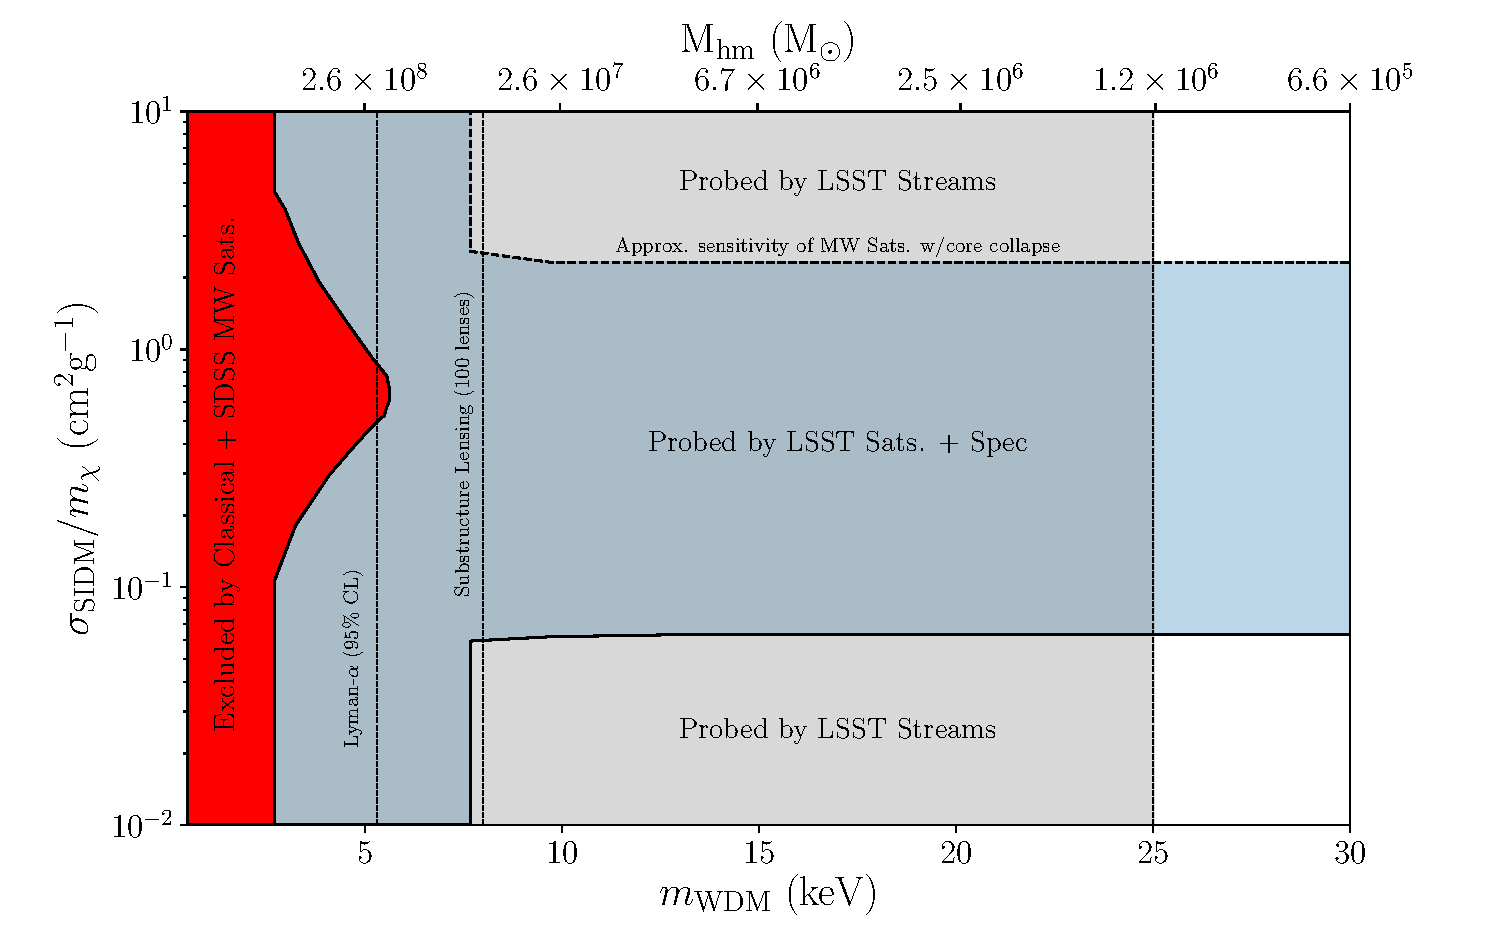
\includegraphics[width=0.6\columnwidth]{wdm_sidm.pdf}
\caption{Warm dark matter mass vs self-interacting dark matter cross section. Two fundamental characteristics of dark matter that are best probed with astrophysics. \EON{N.B. even though there is a degeneracy between SIDM/WDM when considering subhalo counts and profiles, it might be possible to break this degeneracy using the fact that halos form later in WDM -- see Bozek+18 for hydro simulation results.}}
\end{figure}

\subsection{Dark Matter-Baryon Scattering \Contact{Vera}}
\Contributors{Vera, Kim,...}
\label{sec:dmbaryon}
In the standard WIMP scenario, dark matter (DM) may be directly observable through its scattering with SM particles.
Direct detection experiments search for DM particles in the Galactic halo scattering with target nuclei, and they achieve exquisite sensitivity, in part from being placed deep underground to provide shielding from cosmic ray backgrounds.
However, given the null results from these experiments, it is important to explore parameter space that is outside the standard WIMP region.
Cosmological and astrophysical observables are unique and robust probes of these complementary regions of parameter space. 
While laboratory searches of DM typically rely on the detailed form of the interaction, the momentum transfer between cosmological fluids is only sensitive to the velocity dependence of the cross section, making these observations very broad and generic probes of DM physics.

In the early Universe, scattering results in the exchange of momentum between the DM and the baryon fluids.
The momentum transfer induces a drag force, which suppresses structure more at progressively smaller scales. 
The effect of scattering is qualitatively similar to a cutoff in the matter power spectrum arising in the WMD and SIDM scenarios; see Figure \ref{fig:dmbaryon_pk} for illustration.
This feature can be sought with tracers of matter on all observable scales. 
The best cosmological and astrophysical limits so far come from CMB temperature, polarization, and lensing anisotropy~\citep{Boddy:2018kfv,Gluscevic:2017ywp,Boddy:2018wzy,Xu:2018efh,Slatyer:2018aqg}, cosmic-ray \cite{}, and Lyman-$\alpha$-forest measurements~\citep{Dvorkin:2013cea,Xu:2018efh}. 
LSST observables will cover a much broader range of scales and can thus substantially extend sensitivity to DM-baryon scattering: substructure measurements from gaps in stellar streams, galaxy strong lensing, dwarf galaxies in the local volume, and weak galaxy lensing. 

\begin{figure}
\centering
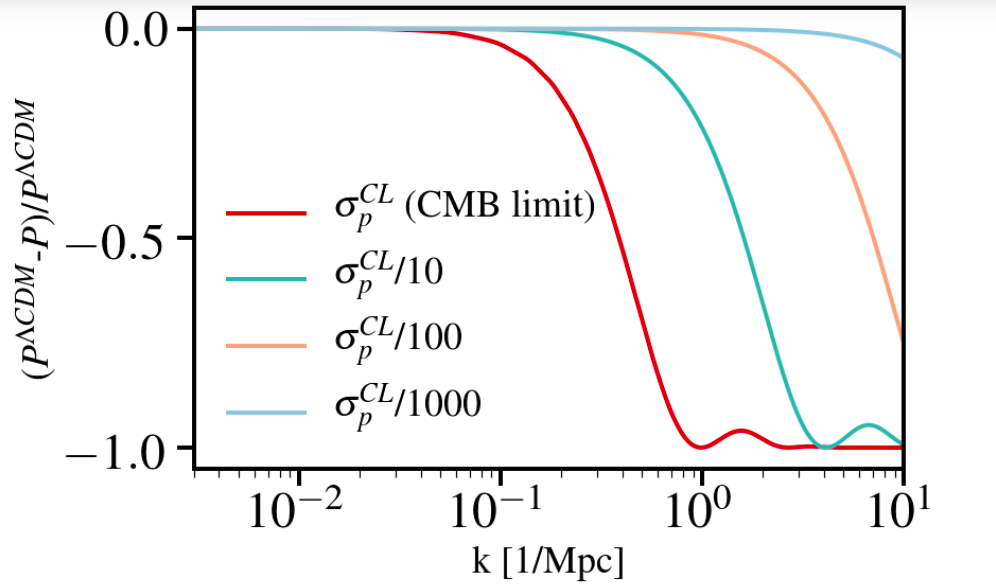
\includegraphics[width=0.6\columnwidth]{figures/dmbaryon_pk.png}
\caption{Linear matter power spectrum at $z=0$. Shown are the residuals between the $CDM$ case and the case where there are velocity-independent spin-independent interactions between DM and protons; DM particle mass is set to 1 MeV, and all other cosmological parameters are set to their best-fit Planck 2015 values. Different residuals display cutoff at different angular scale, controlled by the magnitude of the interaction cross section. The highest cross section shown corresponds to the current upper limit inferred from analyses of Planck data \citep{Gluscevic:2017ywp,Boddy:2018kfv}.}
\label{fig:dmbaryon_pk}
\end{figure}
As an example, a measurement of the minimum halo mass translates into an upper limit on DM-proton interaction cross section, based on the corresponding cutoff in the  matter power spectrum; Figure \ref{fig:dmbaryon_pk} shows how the position of the cutoff in the linear $P(k)$ varies as a function of the interaction cross section. For example, a lower limit on the cutoff of $k_\text{cutoff}\sim 10$ roughly corresponds to an upper limit on the cross section which is 100 times more stringent than the current limit from CMB searches for DM scattering. Using limits on WDM as a proxy for a suppressed $P(k)$, and the illustration in Figure \ref{fig:dmbaryon_pk} to guide the eye, a minimum halo mass of $10^8$ solar masses would imply more than three orders of magnitude improvement over the current cosmological limit on the interaction cross section.

\subsection{Field Dark Matter \Contact{Chanda}}
\label{sec:axions}

Fuzzy dark matter: In this scenario, dark matter is made of ultra light scalar particles with mass around $10^{-22}~{\rm eV}$. With such as a small mass, the de Broglie wavelength of the dark matter particle is $\mathcal{O}({\rm kpc})$, comparable to galaxy sizes, and the quantum effect becomes relevant in structure formation. Fuzzy dark matter predicts a solitonic core in the halo center and its size is set by the de Broglie wavelength of the dark matter particle. On larger scales, the structure predicted in fuzzy dark matter is less clumpy and less abundant than its CDM counterpart due to the quantum interference effect. 

\section{Field Dark Matter \Contact{Chanda}}
\label{sec:axions}

While current observations of the matter power spectrum constrain the minimum mass of thermally produced dark matter, other mechanisms can  produce dark matter with significantly lower masses. The landscape of light dark matter candidates is vast, and in this section, we specifically focus on the class of axion-like particle (ALP) dark matter candidates.
ALP models span a wide range of viable parameter space (both in coupling strength and mass), and many of the observables described in this section can be generically applied to a broader class of light scalar particles.

The ALP paradigm was inspired by the QCD axion, which arises as a by-product of the most successful solution to the Strong CP Problem in the Standard Model \citep{PecceiQuinn:1977}. 
The cosmological abundance of axions is set by the Peccei-Quinn symmetry breaking scale, $f_\phi$, with a value
\begin{equation}
\Omega_\phi\sim\left(\frac{f_\phi}{10^{11-12}\,{\rm GeV}}\right)^{7/6}.
\end{equation}
This expression may be altered due to the temperature-dependence of the axion mass and ignorance about whether the Peccei-Quinn symmetry breaks before or after inflation. 
QCD theory gives no {\it a priori} prediction for the axion mass; however, in the context of dark matter composed of QCD axions, the axion mass is considered to be $m_\phi< 10^{-3}$ eV ($10^{-39}$ kg). 
If the initial misalignment angle is order unity, this yields a QCD axion mass of $m_\phi \sim 10^{-5}$ eV ($10^{-41}$ kg).
%\ADW{Please check Chanda!}
The broader category of ALPs possess QCD-axion-like potentials producing light scalar particles that obey a shift symmetry ($\phi \rightarrow \phi + 2\pi n$), but do not obey the same coupling between particle mass and symmetry breaking scale. 
ALPs can be motivated by string theory, where there are many moduli with axion-like potentials, and can produce a range of astrophysical phenomenology.
%ALPs can be sufficiently different from the QCD axion so as to produce notably different astrophysical phenomenology. 
ALPs may be non-thermally produced in the early universe and survive as a cold dark matter population until today \citep[\eg][]{Arias:2012az}.

%Fuzzy dark matter: In this scenario, dark matter is made of ultra light scalar particles with mass around $10^{-22}~{\rm eV}$. With such as a small mass, the de Broglie wavelength of the dark matter particle is $\mathcal{O}({\rm kpc})$, comparable to galaxy sizes, and the quantum effect becomes relevant in structure formation. Fuzzy dark matter predicts a solitonic core in the halo center and its size is set by the de Broglie wavelength of the dark matter particle. On larger scales, the structure predicted in fuzzy dark matter is less clumpy and less abundant than its CDM counterpart due to the quantum interference effect.

Astrophysical observations place the only known lower bound on the mass of ALPs and other non-thermally produced ultra-light particles, commonly described as ``fuzzy'' dark matter \citep[FDM; \eg,][]{Hu:2000,Hui:2017}. 
The de Broglie wavelength of these particles is constrained to be smaller than the size of the smallest galaxy, $\mathcal{O}(1\kpc)$, setting a lower limit on particle mass at $m_\phi \gtrsim 10^{-22}$ eV. 
%The formation of halos with mass $M_h \lesssim 10^{10} (m_\phi / 10^{-22} \eV)^{-4/3} \Msun$ will be significantly suppressed, and halos with $M_h \lesssim 10^7 (m_\phi / 10^{-22} \eV)^{-3/2} \Msun$ should not form at all \citep{Hui:2017}.
In addition, FDM is predicted to produce solitonic cores in the centers of halos, which would measurably effect the velocity profiles of dark-matter dominated galaxies \citep{Robles:2012uy,Robles:2018fur,Schive:2014hza,Du:2016aik}. 
On larger scales, the structure predicted in FDM is less abundant than its CDM counterpart due to quantum interference effects.
This is similar to the case of WDM, and again dark matter properties can be constrained through mesurements of the least massive dark matter halos.
Combining Equation 8 of \citet[][]{1703.09126} with \eqnref{Mhm} in \secref{wdm}, we can express constraints on the minimum FDM mass, $m_\phi$, as a function of the half-mode halo mass, $M_{\rm hm}$:
\begin{equation}
M_{\rm hm} = 1.2 \times 10^{11} \left( \frac{m_\phi}{10^{-22}\eV} \right)^{-1.4} \Msun,
\end{equation}
or expressed in terms of $m_\phi$, 
\begin{equation}
m_\phi = 3.1 \times 10^{-21} \left( \frac{M_{\rm hm}}{10^{9}\Msun} \right)^{-0.71} \eV.
\end{equation}
LSST will constrain the minumum mass of light bosonic dark matter to be greater than $m_\phi \sim 10^{-20} \eV$ by precisely constraing the half-mode mass to be less than $M_{\rm hm} \sim 10^{8} \Msun$.

%ADW: I think the paragraphs below have slightly too much much detail, for this report. It would be good to talk about axion stars, galaxy caustics, and anomalous energy loss in stellar populations and SN.
%CPW, 10/29/2018: I think some of it should be reintroduced, but I have shortened and edited to suggest these are different scenarios under consideration.
%Sikivie & Yang 2009

There has been significant debate in the literature about the astrophysical phenomenology of the QCD axion and ALPs.
\citet{Sikivie:2009} noted that because the axion is a scalar with high abundance in the early universe (circa matter-radiation equality), the axion could potentially settle into a Bose-Einstein condensate (BEC) state, whereby all particles can be described using one coherent ground state wave function. 
Furthermore, \citet{Sikivie:2009} argue that during the radiation-dominated era, axions will rethermalize into BECs with a Hubble-scale correlation length.
This could produce significant observational implications, such as several-kpc-scale caustic structures observable in the stellar distributions of the Milky Way and other low-redshift galaxies \citep[\eg,][]{Natarajan:2006,0805.4556,Rindler-Daller:2013zxa}.

On the other hand, \citet{1412.5930} argue that a particle such as the QCD axion, which has an attractive self-interaction, in an attractive gravitational potential will not sustain Hubble-scale correlations.
Instead, \citet{1412.5930} predict that axions will form coherent clumps that have been called ``Axion stars'' or ``Bose stars'' \citep[\eg][]{Kolb:1993}.\footnote{For the QCD axion it would be more appropriate to call these ``axteroids'' (a term coined by Anna Watts) due to their mass of $\roughly 10^{-11} \Msun$ \citep{Tkachev:1991ka,Braaten:2018nag}.} 
Looking beyond the QCD axion, for some ALP models, compact BEC ``miniclusters'' could form and grow to $\gtrsim 1\Msun$, at which point they may be detectable by LSST through mergers with other compact objects \citep{1808.04746} or through microlensing \citep{1707.03310}.

%What is distinct about this proposal is not so much the idea that the axion might begin as a BEC -- this seems likely (although making this statement formal is an open problem) -- but rather once the particles experience perturbations, do they remain in a BEC state? %These are distinct from the spherical topology predicted for WIMPs \citep{Bertschinger:2006nq}. 
%These massive compact structures could be detected through collisions with stellar remnants, which could be constrained by the transient event rate measured by LSST \citep{1808.04746}.
%Still other theories predict that axions could collapse 
%\ADW{I don't know if I believe either of these detection scenarios.}

%This proposal has a distinct phenomenology and LSST observations providing insights into caustics around nearby galaxies, may help distinguish between the two.

%Complicating LSST's capacity to distinguish between models is the possibility of degeneracy between the SY model and other axion-like particle phenomenologies. Both of the aforementioned scenarios, which have kicked off significant debate and renewed interest in Bose-Einstein condensed axion phenomenology, focus on the QCD axion in a mass range of around $10^{-5}$ eV. There is an extensive literature regarding axion phenomenology beyond the QCD axion and this mass range, e.g. ultralight axions (ULA) and fuzzy dark matter (FDM). In ULA/FDM scenarios, the De Broglie wavelength of the particle is such that the coherent wave can be halo-scale, which may give distinct stellar density distributions, which LSST will measure, than the SY proposal or the clump scenario.

Additional astrophysical constraints on ALPs generally come from proposed couplings with photons and/or electrons. 
For example, the Lagrangian can be expressed as,
\begin{equation}
    \mathcal{L} = -\frac{1}{2} \partial_\mu\phi\partial^\mu\phi + \frac{1}{2}m_\phi^2 \phi^2 - \frac{1}{4}g_{\phi\gamma}F_{\mu\nu}\tilde{F}^{\mu\nu}\phi - g_{\phi e}\frac{\partial_\mu\phi}{2m_e}\bar{\psi}_e \gamma^\mu\gamma_5\psi_e,
\end{equation}
where $g_{\phi\gamma}$ is the photon-axion coupling, $g_{\phi e}$ is the axion-electron coupling, $F^{\mu\nu}$ is the electromagnetic field tensor (and $\tilde{F}$ its dual), and $\psi_e$ is the electron field \citep[\eg][]{1302.6283,Redondo:2013wwa}.\footnote{Additional couplings to nucleons are allowed, but are not relevant for the LSST observations discussed here.}
For sufficiently large couplings to photons or electrons, the ALP can manifest as an additional anomalous energy loss mechanism, transporting energy out of the interiors of stars \citep[\eg,][]{Raffelt:1990}.
This energy loss could affect the evolution of stars, for example altering the lifetimes of giant stars \citep{Ayala:2014,Viaux:2013hca,Viaux:2013lha} or the cooling rate of white dwarf stars \citep{Isern:2008}.
The precise photometry of LSST will provide sensitive measurements of stellar populations to search for deviations from the predictions of standard stellar evolutionary models.

\begin{comment}
\TT{We should also mention the dark photon}
\ADW{Would we want to include some discussion of soliton cores from fuzzy DM?}

LSST will be able to probe axion dark matter in the following ways:
\begin{itemize}
    \item Caustics around Nearby Galaxies \CPW{11.25 Dealt with, now?}
    \item Anomalous Cooling in Stellar Populations 
    \begin{itemize}
        \item White dwarf luminosity function
        \item Globular cluster
        \item Cepheids / blue loop?
    \end{itemize}
    \item Supernova Observations
    
\end{itemize}
\end{comment}




% Axion dark matter: The QCD axion arises as a by-product of the most successful solution to the Strong CP Problem in the Standard Model \citep{PecceiQuinn:1977}. 
% The abundance of axions is set by the Peccei-Quinn symmetry breaking scale $f_a$ with a value
% \begin{equation}
% \Omega_a\sim\left(\frac{f_a}{10^{11-12}\,{\rm GeV}}\right)^{7/6}.
% \end{equation}
% This expression may be altered due to the temperature-dependence of the axion mass and ignorance about whether the Peccei-Quinn symmetry breaks before or after inflation. 
% Axion theory gives no {\it a priori} prediction for the axion mass; however, in the context of dark matter composed of QCD axions, an axion mass $m_\phi< 10^{-3}$ eV ($10^{-39}$ kg). 
% If the initial mass alignment angle is order unity, this yields a QCD axion mass of $\roughly 10^{-5}$ eV ($10^{-41}$ kg) is usually considered.  \ADW{Please check Chanda!}

% A broader category of axion-like particles (ALPs) possess QCD axion-like potentials, but do not obey the same coupling between particle mass and symmetry breaking scale. ALPs are a broad class of light scalar particles which obey a shift symmetry $\phi \rightarrow \phi + 2\pi n$. They can be motivated by string theory, where there are many moduli with axion-like potentials. ALPs can be sufficiently different from the QCD axion so as to produce notably different astrophysical phenomenology. 

% Astrophysical constraints on ALPs generally come from a hypothetical coupling of the ALP with photons and/or electrons. 
% \begin{equation}
%     \mathcal{L} = -\frac{1}{2} \partial_\mu\phi\partial^\mu\phi + \frac{1}{2}m_\phi^2 \phi^2 - \frac{1}{4}g_{\phi\gamma}F_{\mu\nu}\tilde{F}^{\mu\nu}\phi,
% \end{equation}
% \ADW{Please check Chanda! -- Do we want all terms? What about couplings to electrons and nucleons?}
% where $g_\phi\gamma$ is the photon-axion coupling and $F^{\mu\nu}$ is the electromagnetic field tensor (and $\tilde{F}$ its dual). 
% In these cases, the production of ALPs in hot, dense environments can result in an anomalous energy loss mechanism as the ALPs escape these environments nearly uninhibited. The existence of such non-standard energy loss can be constrained through 

% Astrophysical observations place the only known lower bound on the mass of ALPs and other non-thermally produced particles, commonly described as ``fuzzy'' dark matter. The Compton wavelength of these particles is constrained to be smaller than the size of the smallest galaxy, setting a lower limit on particle mass at $m \gtrsim 10^{-22}$ eV. The scalar nature of the axion along with its high abundance in the early universe can -- what was the rest of this sentence? The mass of the particle also determines the significance of quantum pressure in structure formation.



% %ADW: I think the paragraphs below have slightly too much much detail, for this report. It would be good to talk about axion stars, galaxy caustics, and anomalous energy loss in stellar populations and SN.

% %CPW, 10/29/2018: I think some of it should be reintroduced, but I have shortened and edited to suggest these are different scenarios under consideration.
% \subsubsection{Axions and Structure Formation}
% There has been significant debate in the literature about the astrophysical phenomenology of the QCD axion. Sikivie and Yang (2009) noted that because the axion is a scalar with high abundance in the early universe (circa matter-radiation equality), the axion could potentially settle into a Bose-Einstein condensate state. By ``Bose-Einstein condensate'' one has loosely meant that all particles can be described using one coherent ground state wave function. What is distinct about Sikivie and Yang's proposal is not so much the idea that the axion might begin as a BEC -- this seems likely (although making this statement formal is an open problem) -- but rather once the particles experience perturbations, do they remain in a BEC state? SY argue that during the radiation-dominated era, axions will rethermalize into BECs with a Hubble-scale correlation length, with significant phenomenological implications such as low-redshift galaxy scale (tens of kpc) caustics with a non-spherical topology. These are distinct from the spherical topology predicted by Bertschinger for WIMPs. 

% \citet{1412.5930} showed that rather than a Hubble-scale correlation length at matter-radiation equality that leads to galaxy halo phenomenology, a particle such as the QCD axion, which has an attractive self-interaction, in an attractive gravitational potential will not stably have large scale correlations. Rather, axions in this early universe era will form clumps that have been called Axion stars or Bose stars (see Kolb and Tkachev 2000) but should more reasonably probably be called axteroids (originating with Anna Watts). This proposal has a distinct phenomenology and LSST observations of rotation curves, providing insights into caustics around nearby galaxies, may help distinguish between the two.

% Complicating LSST's capacity to distinguish between models is the possibility of degeneracy between the SY model and other axion-like particle phenomenologies. Both of the aforementioned scenarios, which have kicked off significant debate and renewed interest in Bose-Einstein condensed axion phenomenology, focus on the QCD axion in a mass range of around $10^{-5}$ eV. There is an extensive literature regarding axion phenomenology beyond the QCD axion and this mass range, e.g. ultralight axions (ULA) and fuzzy dark matter (FDM). In ULA/FDM scenarios, the De Broglie wavelength of the particle is such that the coherent wave can be halo-scale. 
% \CPW{IS IT CLEAR THAT THIS WILL ALWAYS GIVE A DIFFERENT CAUSTIC STRUCTURE FROM THE SY PROPOSAL?}
% \ADW{Would we want to include some discussion of soliton cores from fuzzy DM?}

% LSST will be able to probe axion dark matter in the following ways:
% \begin{itemize}
%     \item Caustics around Nearby Galaxies
%     \item Anomalous Cooling in Stellar Populations 
%     \begin{itemize}
%         \item White dwarf luminosity function
%         \item Globular cluster
%         \item Cepheids / blue loop?
%     \end{itemize}
%     \item Supernova Observations
    
% \end{itemize}

% \begin{figure}
% \centering
% 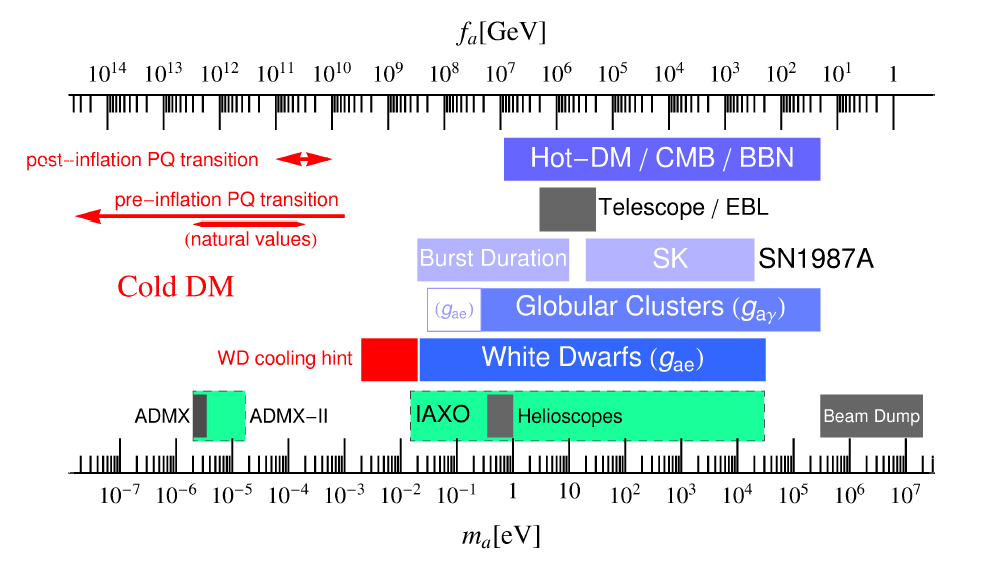
\includegraphics[width=0.6\columnwidth]{axions.png}
% 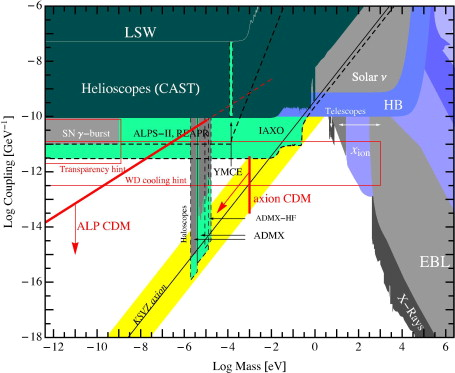
\includegraphics[width=0.39\columnwidth]{alps.jpg}
% \caption{Maybe something like on the left for axion constraints 
% Taken from \citep{Redino:2015} \url{https://arxiv.org/abs/1512.06822}. Right: Figure that could be used for ALP constraints \citep{Ringwald:2012} \url{https://arxiv.org/abs/1210.5081}}
% \end{figure}


\subsection{Compact Objects \Contact{Simeon}}
\Contributors{Will D, Nathan G., Michael M., Simeon, George C.,...}
\label{sec:machos}

\section{Compact Objects \Contact{Simeon}}
\label{sec:machos}
\Contributors{Simeon Bird, Juan Garc\'ia-Bellido, Will Dawson, Nathan Golovich, Michael Medford}
% George Chapline

Compact objects, particularly black holes formed in the early universe, represent one of the oldest and most venerable models of dark matter. Primordial black holes could originate from small-scale density fluctuations during the era of inflation. The same fluctuations that lay down the seeds of galaxies, if boosted on small scales, can lead to some small areas having a Schwarzschild mass within the horizon, which spontaneously collapse to form black holes. Because these black holes do not accrete or radiate strongly (at the time of formation there is no gas to form an accretion disc), they are a natural candidate for dark matter \citep{Carr:1974nx,Meszaros:1974,1975Natur.253..251C,Bellido:1996,Carr:2016drx}. 

Compact object dark matter is fundamentally different from particle models; primordial black holes cannot be studied in an accelerator and can only be detected through their gravitational force. Current constraints suggest that primordial black holes do not make up all of dark matter \citep[\eg][]{Sasaki:2018}. However, these constraints may be evaded if PBHs are spatially clustered \citep{Clesse:2015,Clesse:2017}. Moreover, primordial black holes are one possible source of the merging $30 \Msun$ black holes recently detected by LIGO \citep{Bird:2016,Clesse:2016}. This possibility has rekindled interest in these objects, both as a source of dark matter and in their own right.

Limits on the abundance and mass range of primordial black holes are wholly observational. The black hole mass is set by the mass enclosed within the horizon at the time of black hole collapse and thus ranges between $10^{-18} \Msun$ ($10^{15}\g$), below which the black hole would evaporate, and $10^9 \Msun$ ($10^{42}\g$), above which structure formation, Big Bang Nucleosynthesis and the formation of the microwave background would be severely affected \citep{Sasaki:2018}. 
For stellar mass black holes, the gold standard for detecting compact objects is microlensing. Current microlensing constraints set limits on the black hole abundance at the level of $10\%$ for black holes $0.01 - 10 \Msun$ \citep[however, see][]{2018MNRAS.479.2889C}. LSST will revolutionize the astrometric microlensing technique,  constraining the abundance of primordial black holes to a level of $10^{-4}$ of the dark matter over a wide range of masses (\secref{compact_objects}).

As primordial black holes form directly from the primordial density fluctuations, a measurement of their abundance would directly constrain the amplitude of density fluctuations \citep{Carr:1974nx, Meszaros:1974}. %1203.2681 
Although these constraints are several orders of magnitude weaker than, for example, those from the microwave background, they probe small scales between $k = 10^{7} - 10^{19}$ $h$/Mpc, much smaller than those measured by other current and future probes \citep{Bringmann:2012}. Because these scales are highly non-linear in the late-time universe, there is no other possible constraint; the information present at early times has been washed away by gravitational evolution. Primordial black holes are thus a probe of primordial density fluctuations in a range that is inaccessible to other techniques~\citep{Josan:2009,Bellido:2017,Bellido:2018}. These curvature fluctuations are imprinted on space-time hypersurfaces during inflation, at extremely high energies, beyond those currently accessible by terrestrial and cosmic accelerators. 
Our understanding of the universe at these high energies, of order $10^{15} \GeV$ and above, comes predominantly from extrapolations of known physics at the electroweak scale.
%At these high energies, of order $10^{15} \GeV$ and above, there are few theoretical constraints, and most of our assumptions come from extrapolations of known physics at the electroweak scale. 
Measurements of the primordial density fluctuations via the abundance of primordial black holes would provide unique insights into physics at these ultra-high energies.

%For example, the long lever of scales means that the constraints on simple scale-invariant inflation models expressed in terms of a scalar index, $n_s$ and a running, $\alpha_s$ can be competitive for some models. 

Furthermore, it may be possible for LSST to constrain the existence of ultra-compact mini-halos using correlated microlensing signals \citep{erickcek2011,li2012}. These objects arise from initial overdensities that are too small to collapse into primordial black holes. These overdensities still collapse at high redshift to form low-mass halos; thus, since these objects form early and have few mergers \citep{Bringmann:2012,Delos:2018}, they have a high concentration and a steeper internal density profile than the standard Navarro-Frenk-White shape. In turn, this makes them easier to detect via lensing and harder to disrupt than standard CDM subhalos. Current constraints on these objects are highly model-dependent. In particular, they largely come from counting gamma-ray photons from astrophysical sources under the assumption of a WIMP dark matter annihilation cross-section. LSST will place new constraints on the existence of small halos via micro-lensing and thereby constrain the physics of the inflaton on scales of $k = 10 \textup{--} 10^7 h$/Mpc for the first time in a model-independent way.

%See Figure 6 of Bringmann 2012: \url{https://arxiv.org/abs/1110.2484}
%Sasaki 2018: \url{https://arxiv.org/abs/1801.05235}


% All of the following tex should be included in the machos.tex. Plus more edits have been made there.

% \begin{figure}
% \centering
% 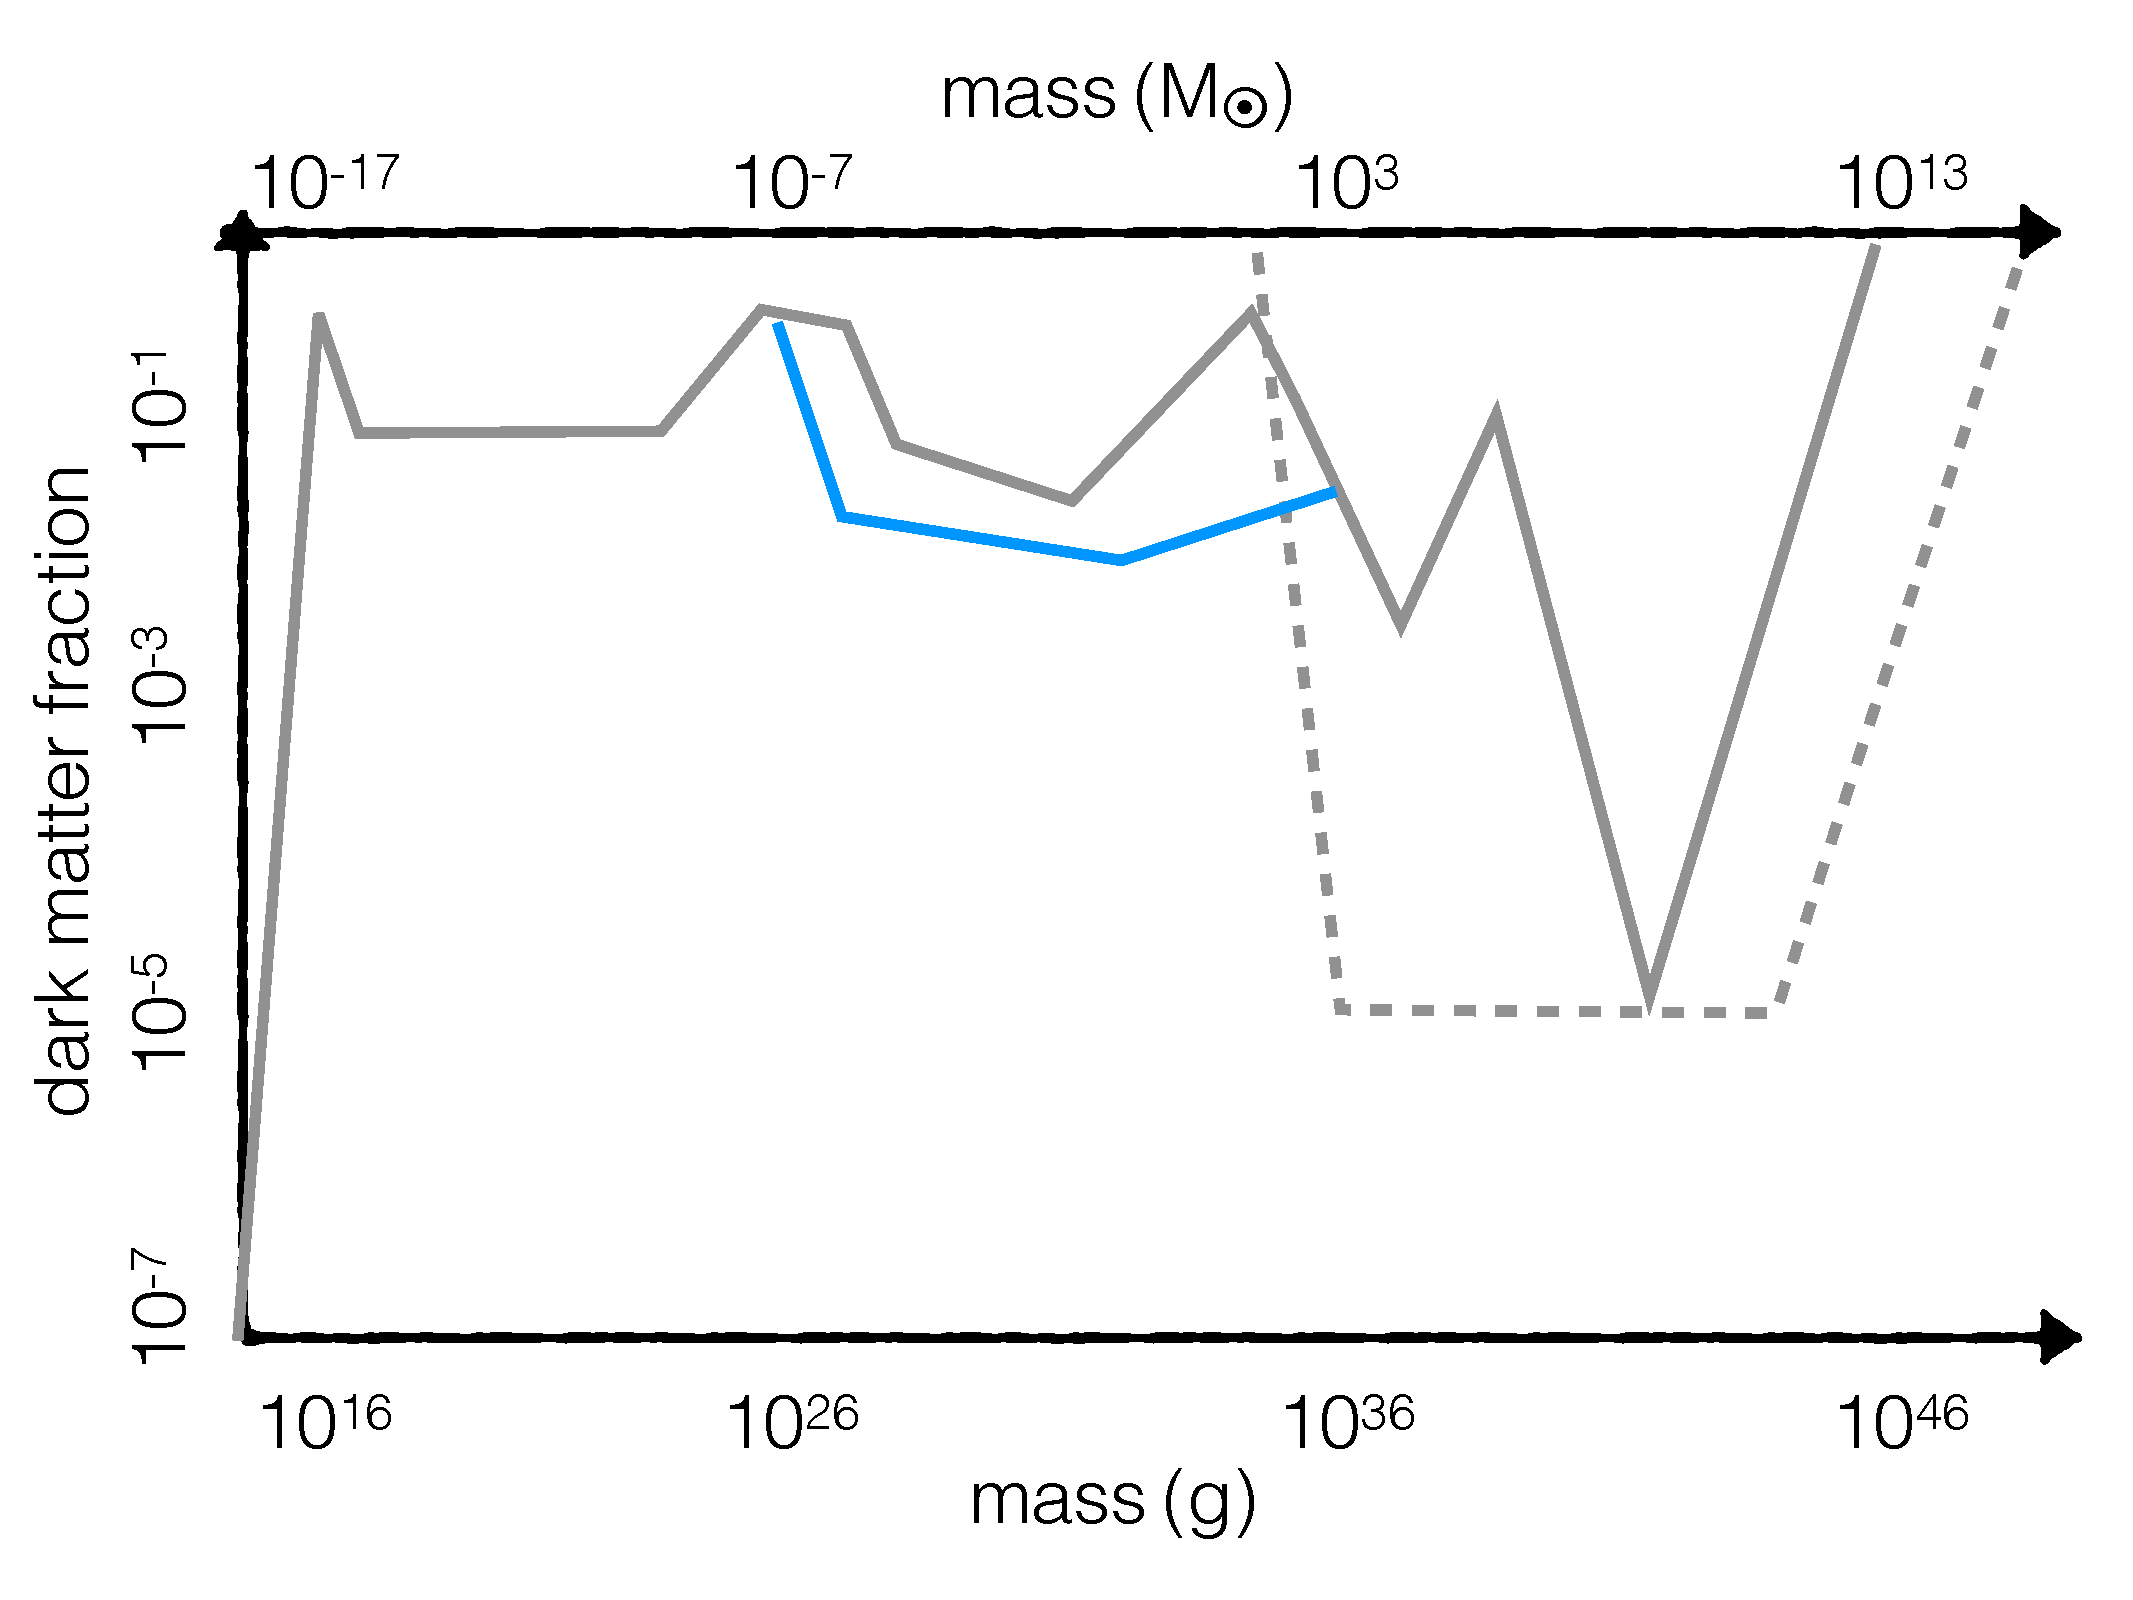
\includegraphics[width=0.6\columnwidth]{macho_cartoon.pdf}
% \caption{Fraction of dark matter that can be accounted for in compact objects.}
% \end{figure}

% Dark matter from compact objects, in particular black holes formed in the early universe, is one of the oldest and most venerable dark matter models. These black holes originate from small-scale density fluctuations during the era of inflation. The same fluctuations that lay down the seeds of galaxies, if boosted on small scales, can lead to some small areas having a Schwarzchild mass within the horizon, which  spontaneously collapses to form black holes. Because these black holes are non-interacting (at time of formation, there is no gas to form an accretion disc) they are a natural candidate for dark matter. 

% Compact halo object dark matter is fundamentally different from particle models; black holes cannot be formed in an accelerator and can only be detected through their gravitational force. Current constraints suggest that primordial black holes make up at most $10\%$ of the dark matter. However, one possible source of the merging $30 M_\odot$ black holes recently detected by LIGO is primordial black holes \cite{Bird:2016}. This possibility has rekindled interest in these objects, both as a source of dark matter and in their own right.

% Limits on the abundance and mass range of primordial black holes are thus wholly observational. The black hole mass is set by the mass enclosed within the horizon at time of black hole collapse and thus ranges between $10^{15}$ g ($10^{-18} M_\odot$), below which the black hole would evaporate, to $10^{42}$ g  ($10^9 M_\odot$), above which structure formation, big bang nucleosynthesis and the formation of the microwave background would be severely affected \cite{Sasaki:2018}. 
% The gold standard technique for detecting compact objects is astrometric microlensing. Current constraints set limits on the black hole abundance at the level of $10\%$ through almost all of the possible mass range, although some constraints are model-dependent. LSST would be able to revolutionize this picture,  constraining the abundance of primordial black holes to a level of $10^{-4}$ of the dark matter through a wide range of masses (see Section \ref{sec:compact_object_abundance}).

% The density fluctuations which seed primordial black holes are on scales much smaller than those measured by other cosmological structures and thus probe a period of inflation several e-foldings later. Given the high energy and uncertainty of inflationary physics, there are few theoretical constraints on the number density and mass of the primordial black holes. Conversely, measurements of the abundance of compact objects such as primordial black holes are the only current constraints on dynamics of inflation on small scales \cite{Bringmann:2012}. Measurements of the abundance of these objects, even if they are only a fraction of the dark matter, thus provides a constraint on the inflationary power spectrum.

% Although these constraints are several orders of magnitude weaker than, for example, those from the microwave background, they probe small scales between $k = 10^{7} - 10^{19}$ h/Mpc, much smaller than those measured by other current and future probes. The long lever of scales means that the constraints on simple scale-invariant inflation models expressed in terms of a scalar index, $n_s$ and a running, $\alpha_s$ can be competitive for some models. Because these scales are highly non-linear in the late-time universe, there is no other possible constraint; the information present at early times has been washed away by gravitational evolution. Primordial black holes thus provide a unique constraint on the matter power spectrum from inflation.

% Furthermore, it may be possible for LSST to constrain the existence of ultra-compact mini-halos using correlated microlensing signals. These objects arise from initial overdensities not large enough to collapse to a primordial black hole. These overdensities still collapse, at high redshift to form low-mass halos. As these objects form early and have few mergers \cite{Delos:2018}, they have a high concentration and a steeper internal density profile than the standard Navarro-Frenk-White shape, making them easier to detect via lensing and harder to disrupt than standard subhalos.

% Current constraints on these objects are highly model-dependent; they come from assuming a WIMP dark matter annihilation cross-section and counting gamma ray photons. LSST would place wholly new constraints on the existence of small halos from micro-lensing, and thus constrain the physics of the inflaton on scales of $k = 10 - 10^7 $ h/Mpc for the first time in a model-independent way.


 
% \subsection{Warm dark matter (WDM)}
% \label{sec:wdm}
% The warm dark matter candidate a long free-streaming length, resulting in a cutoff on halo abundance for low-mass halos. In the warm dark matter theory, dark matter typically has a light mass such that it decouples from the thermal bath late and lead to a long free-streaming length.

% In the standard thermal dark matter paradigm, primordial inhomogeneities in the matter density field are washed out by collisional damping and free streaming of particle dark matter \citep{Hofmann:2001,Green:2003un, Bertschinger:2006nq, Loeb:2005pm}.  For a canonical 100-GeV thermal relic dark matter particle, these processes erase cosmological perturbations with $M \leq 10^{-6} \Msun$ \citep[i.e., Earth mass][]{Green:2003un}. Lighter particles continue to free stream at lower temperatures (later times), thus suppressing the formation of structure at higher mass scales.

% Free-streaming also sets the low-mass end of clustering in sterile neutrino dark matter models, which decouple from the primordial plasma while they are relativistic. In this case, the free-streaming scale can be approximated by the (comoving) size of the horizon when the sterile neutrinos become nonrelativistic. The comoving horizon size at $z = 10^7$ corresponds to $m = 2.5 \keV$, and is approximately $50 \kpc$, which is significantly smaller than the scale derived above for $\Lstar$ galaxies (Adhikari et al. 2017). 

% Astrophysical constraints are generally placed on warm dark matter by observing the smallest gravitationally bound dark matter halos.  The half-mode scale, the scale at which the dark matter transfer function is reduced by half, represents a characteristic halo mass scale where observations can be performed. 
% The half-mode halo mass, $M_{hm}$, is related to the WDM particle mass, $m_{\rm WDM}$, by \citep{Bullock:2017xww}
% \begin{equation}
%     M_{\rm hm} = 5.5 \times 10^{10} \big ( \frac{m_{\rm WDM}}{1 {\rm keV}} \big)^{-3.33} {\rm M_\odot}.
% \end{equation}
% Thus, an observed suppression in the abundance of dark matter halos smaller than a given scale, $M_{hm}$, could signify the existence of a thermal dark matter particle with mass,
% \begin{equation}
%     m_{\rm WDM} =  3.33 \big ( \frac{M_{hm}}{10^{9} {\rm M_\odot}} \big)^{-0.3} {\rm keV}
% \end{equation}

% \begin{figure}
% \centering
% 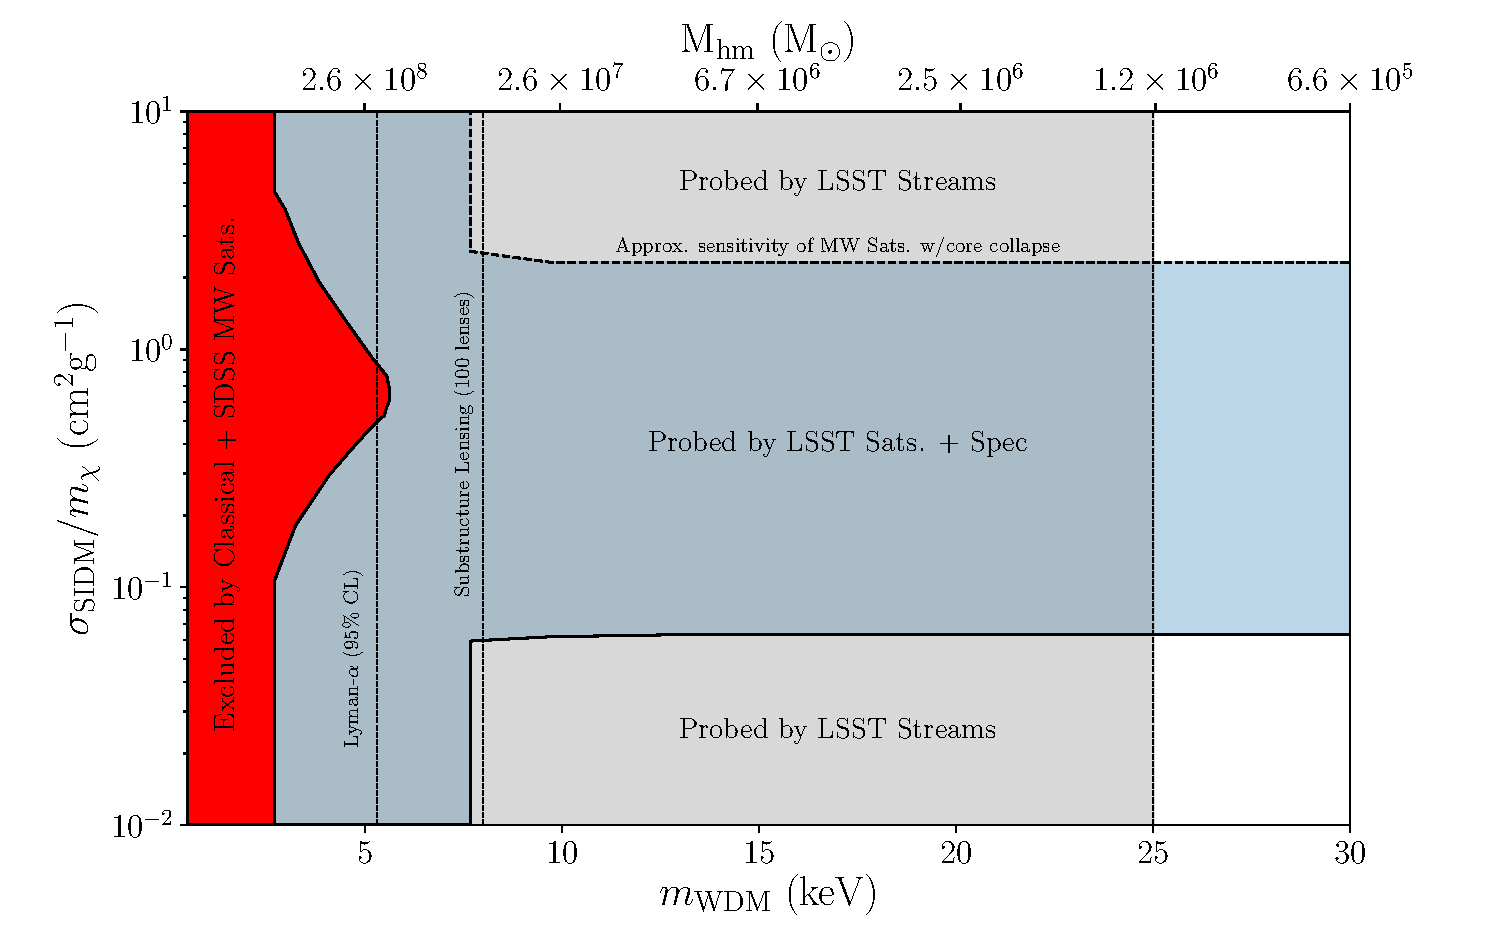
\includegraphics[width=0.6\columnwidth]{wdm_sidm.pdf}
% \caption{Warm dark matter mass vs self-interacting dark matter cross section. Two fundamental characteristics of dark matter that are best probed with astrophysics.}
% \end{figure}

% \subsection{Primordial Black Holes \Contributors{Will D, Nathan G., Michael M., Simeon, ...}}
% \label{sec:machos}

% \section{Compact Objects \Contact{Simeon}}
\label{sec:machos}
\Contributors{Simeon Bird, Juan Garc\'ia-Bellido, Will Dawson, Nathan Golovich, Michael Medford}
% George Chapline

Compact objects, particularly black holes formed in the early universe, represent one of the oldest and most venerable models of dark matter. Primordial black holes could originate from small-scale density fluctuations during the era of inflation. The same fluctuations that lay down the seeds of galaxies, if boosted on small scales, can lead to some small areas having a Schwarzschild mass within the horizon, which spontaneously collapse to form black holes. Because these black holes do not accrete or radiate strongly (at the time of formation there is no gas to form an accretion disc), they are a natural candidate for dark matter \citep{Carr:1974nx,Meszaros:1974,1975Natur.253..251C,Bellido:1996,Carr:2016drx}. 

Compact object dark matter is fundamentally different from particle models; primordial black holes cannot be studied in an accelerator and can only be detected through their gravitational force. Current constraints suggest that primordial black holes do not make up all of dark matter \citep[\eg][]{Sasaki:2018}. However, these constraints may be evaded if PBHs are spatially clustered \citep{Clesse:2015,Clesse:2017}. Moreover, primordial black holes are one possible source of the merging $30 \Msun$ black holes recently detected by LIGO \citep{Bird:2016,Clesse:2016}. This possibility has rekindled interest in these objects, both as a source of dark matter and in their own right.

Limits on the abundance and mass range of primordial black holes are wholly observational. The black hole mass is set by the mass enclosed within the horizon at the time of black hole collapse and thus ranges between $10^{-18} \Msun$ ($10^{15}\g$), below which the black hole would evaporate, and $10^9 \Msun$ ($10^{42}\g$), above which structure formation, Big Bang Nucleosynthesis and the formation of the microwave background would be severely affected \citep{Sasaki:2018}. 
For stellar mass black holes, the gold standard for detecting compact objects is microlensing. Current microlensing constraints set limits on the black hole abundance at the level of $10\%$ for black holes $0.01 - 10 \Msun$ \citep[however, see][]{2018MNRAS.479.2889C}. LSST will revolutionize the astrometric microlensing technique,  constraining the abundance of primordial black holes to a level of $10^{-4}$ of the dark matter over a wide range of masses (\secref{compact_objects}).

As primordial black holes form directly from the primordial density fluctuations, a measurement of their abundance would directly constrain the amplitude of density fluctuations \citep{Carr:1974nx, Meszaros:1974}. %1203.2681 
Although these constraints are several orders of magnitude weaker than, for example, those from the microwave background, they probe small scales between $k = 10^{7} - 10^{19}$ $h$/Mpc, much smaller than those measured by other current and future probes \citep{Bringmann:2012}. Because these scales are highly non-linear in the late-time universe, there is no other possible constraint; the information present at early times has been washed away by gravitational evolution. Primordial black holes are thus a probe of primordial density fluctuations in a range that is inaccessible to other techniques~\citep{Josan:2009,Bellido:2017,Bellido:2018}. These curvature fluctuations are imprinted on space-time hypersurfaces during inflation, at extremely high energies, beyond those currently accessible by terrestrial and cosmic accelerators. 
Our understanding of the universe at these high energies, of order $10^{15} \GeV$ and above, comes predominantly from extrapolations of known physics at the electroweak scale.
%At these high energies, of order $10^{15} \GeV$ and above, there are few theoretical constraints, and most of our assumptions come from extrapolations of known physics at the electroweak scale. 
Measurements of the primordial density fluctuations via the abundance of primordial black holes would provide unique insights into physics at these ultra-high energies.

%For example, the long lever of scales means that the constraints on simple scale-invariant inflation models expressed in terms of a scalar index, $n_s$ and a running, $\alpha_s$ can be competitive for some models. 

Furthermore, it may be possible for LSST to constrain the existence of ultra-compact mini-halos using correlated microlensing signals \citep{erickcek2011,li2012}. These objects arise from initial overdensities that are too small to collapse into primordial black holes. These overdensities still collapse at high redshift to form low-mass halos; thus, since these objects form early and have few mergers \citep{Bringmann:2012,Delos:2018}, they have a high concentration and a steeper internal density profile than the standard Navarro-Frenk-White shape. In turn, this makes them easier to detect via lensing and harder to disrupt than standard CDM subhalos. Current constraints on these objects are highly model-dependent. In particular, they largely come from counting gamma-ray photons from astrophysical sources under the assumption of a WIMP dark matter annihilation cross-section. LSST will place new constraints on the existence of small halos via micro-lensing and thereby constrain the physics of the inflaton on scales of $k = 10 \textup{--} 10^7 h$/Mpc for the first time in a model-independent way.

%See Figure 6 of Bringmann 2012: \url{https://arxiv.org/abs/1110.2484}
%Sasaki 2018: \url{https://arxiv.org/abs/1801.05235}


% \subsection{Axions and Axion-Like Dark Matter \Contributors{Chanda, Esra, ADW, Manuel, ...}}
% \label{sec:axions}


% \section{Field Dark Matter \Contact{Chanda}}
\label{sec:axions}

While current observations of the matter power spectrum constrain the minimum mass of thermally produced dark matter, other mechanisms can  produce dark matter with significantly lower masses. The landscape of light dark matter candidates is vast, and in this section, we specifically focus on the class of axion-like particle (ALP) dark matter candidates.
ALP models span a wide range of viable parameter space (both in coupling strength and mass), and many of the observables described in this section can be generically applied to a broader class of light scalar particles.

The ALP paradigm was inspired by the QCD axion, which arises as a by-product of the most successful solution to the Strong CP Problem in the Standard Model \citep{PecceiQuinn:1977}. 
The cosmological abundance of axions is set by the Peccei-Quinn symmetry breaking scale, $f_\phi$, with a value
\begin{equation}
\Omega_\phi\sim\left(\frac{f_\phi}{10^{11-12}\,{\rm GeV}}\right)^{7/6}.
\end{equation}
This expression may be altered due to the temperature-dependence of the axion mass and ignorance about whether the Peccei-Quinn symmetry breaks before or after inflation. 
QCD theory gives no {\it a priori} prediction for the axion mass; however, in the context of dark matter composed of QCD axions, the axion mass is considered to be $m_\phi< 10^{-3}$ eV ($10^{-39}$ kg). 
If the initial misalignment angle is order unity, this yields a QCD axion mass of $m_\phi \sim 10^{-5}$ eV ($10^{-41}$ kg).
%\ADW{Please check Chanda!}
The broader category of ALPs possess QCD-axion-like potentials producing light scalar particles that obey a shift symmetry ($\phi \rightarrow \phi + 2\pi n$), but do not obey the same coupling between particle mass and symmetry breaking scale. 
ALPs can be motivated by string theory, where there are many moduli with axion-like potentials, and can produce a range of astrophysical phenomenology.
%ALPs can be sufficiently different from the QCD axion so as to produce notably different astrophysical phenomenology. 
ALPs may be non-thermally produced in the early universe and survive as a cold dark matter population until today \citep[\eg][]{Arias:2012az}.

%Fuzzy dark matter: In this scenario, dark matter is made of ultra light scalar particles with mass around $10^{-22}~{\rm eV}$. With such as a small mass, the de Broglie wavelength of the dark matter particle is $\mathcal{O}({\rm kpc})$, comparable to galaxy sizes, and the quantum effect becomes relevant in structure formation. Fuzzy dark matter predicts a solitonic core in the halo center and its size is set by the de Broglie wavelength of the dark matter particle. On larger scales, the structure predicted in fuzzy dark matter is less clumpy and less abundant than its CDM counterpart due to the quantum interference effect.

Astrophysical observations place the only known lower bound on the mass of ALPs and other non-thermally produced ultra-light particles, commonly described as ``fuzzy'' dark matter \citep[FDM; \eg,][]{Hu:2000,Hui:2017}. 
The de Broglie wavelength of these particles is constrained to be smaller than the size of the smallest galaxy, $\mathcal{O}(1\kpc)$, setting a lower limit on particle mass at $m_\phi \gtrsim 10^{-22}$ eV. 
%The formation of halos with mass $M_h \lesssim 10^{10} (m_\phi / 10^{-22} \eV)^{-4/3} \Msun$ will be significantly suppressed, and halos with $M_h \lesssim 10^7 (m_\phi / 10^{-22} \eV)^{-3/2} \Msun$ should not form at all \citep{Hui:2017}.
In addition, FDM is predicted to produce solitonic cores in the centers of halos, which would measurably effect the velocity profiles of dark-matter dominated galaxies \citep{Robles:2012uy,Robles:2018fur,Schive:2014hza,Du:2016aik}. 
On larger scales, the structure predicted in FDM is less abundant than its CDM counterpart due to quantum interference effects.
This is similar to the case of WDM, and again dark matter properties can be constrained through mesurements of the least massive dark matter halos.
Combining Equation 8 of \citet[][]{1703.09126} with \eqnref{Mhm} in \secref{wdm}, we can express constraints on the minimum FDM mass, $m_\phi$, as a function of the half-mode halo mass, $M_{\rm hm}$:
\begin{equation}
M_{\rm hm} = 1.2 \times 10^{11} \left( \frac{m_\phi}{10^{-22}\eV} \right)^{-1.4} \Msun,
\end{equation}
or expressed in terms of $m_\phi$, 
\begin{equation}
m_\phi = 3.1 \times 10^{-21} \left( \frac{M_{\rm hm}}{10^{9}\Msun} \right)^{-0.71} \eV.
\end{equation}
LSST will constrain the minumum mass of light bosonic dark matter to be greater than $m_\phi \sim 10^{-20} \eV$ by precisely constraing the half-mode mass to be less than $M_{\rm hm} \sim 10^{8} \Msun$.

%ADW: I think the paragraphs below have slightly too much much detail, for this report. It would be good to talk about axion stars, galaxy caustics, and anomalous energy loss in stellar populations and SN.
%CPW, 10/29/2018: I think some of it should be reintroduced, but I have shortened and edited to suggest these are different scenarios under consideration.
%Sikivie & Yang 2009

There has been significant debate in the literature about the astrophysical phenomenology of the QCD axion and ALPs.
\citet{Sikivie:2009} noted that because the axion is a scalar with high abundance in the early universe (circa matter-radiation equality), the axion could potentially settle into a Bose-Einstein condensate (BEC) state, whereby all particles can be described using one coherent ground state wave function. 
Furthermore, \citet{Sikivie:2009} argue that during the radiation-dominated era, axions will rethermalize into BECs with a Hubble-scale correlation length.
This could produce significant observational implications, such as several-kpc-scale caustic structures observable in the stellar distributions of the Milky Way and other low-redshift galaxies \citep[\eg,][]{Natarajan:2006,0805.4556,Rindler-Daller:2013zxa}.

On the other hand, \citet{1412.5930} argue that a particle such as the QCD axion, which has an attractive self-interaction, in an attractive gravitational potential will not sustain Hubble-scale correlations.
Instead, \citet{1412.5930} predict that axions will form coherent clumps that have been called ``Axion stars'' or ``Bose stars'' \citep[\eg][]{Kolb:1993}.\footnote{For the QCD axion it would be more appropriate to call these ``axteroids'' (a term coined by Anna Watts) due to their mass of $\roughly 10^{-11} \Msun$ \citep{Tkachev:1991ka,Braaten:2018nag}.} 
Looking beyond the QCD axion, for some ALP models, compact BEC ``miniclusters'' could form and grow to $\gtrsim 1\Msun$, at which point they may be detectable by LSST through mergers with other compact objects \citep{1808.04746} or through microlensing \citep{1707.03310}.

%What is distinct about this proposal is not so much the idea that the axion might begin as a BEC -- this seems likely (although making this statement formal is an open problem) -- but rather once the particles experience perturbations, do they remain in a BEC state? %These are distinct from the spherical topology predicted for WIMPs \citep{Bertschinger:2006nq}. 
%These massive compact structures could be detected through collisions with stellar remnants, which could be constrained by the transient event rate measured by LSST \citep{1808.04746}.
%Still other theories predict that axions could collapse 
%\ADW{I don't know if I believe either of these detection scenarios.}

%This proposal has a distinct phenomenology and LSST observations providing insights into caustics around nearby galaxies, may help distinguish between the two.

%Complicating LSST's capacity to distinguish between models is the possibility of degeneracy between the SY model and other axion-like particle phenomenologies. Both of the aforementioned scenarios, which have kicked off significant debate and renewed interest in Bose-Einstein condensed axion phenomenology, focus on the QCD axion in a mass range of around $10^{-5}$ eV. There is an extensive literature regarding axion phenomenology beyond the QCD axion and this mass range, e.g. ultralight axions (ULA) and fuzzy dark matter (FDM). In ULA/FDM scenarios, the De Broglie wavelength of the particle is such that the coherent wave can be halo-scale, which may give distinct stellar density distributions, which LSST will measure, than the SY proposal or the clump scenario.

Additional astrophysical constraints on ALPs generally come from proposed couplings with photons and/or electrons. 
For example, the Lagrangian can be expressed as,
\begin{equation}
    \mathcal{L} = -\frac{1}{2} \partial_\mu\phi\partial^\mu\phi + \frac{1}{2}m_\phi^2 \phi^2 - \frac{1}{4}g_{\phi\gamma}F_{\mu\nu}\tilde{F}^{\mu\nu}\phi - g_{\phi e}\frac{\partial_\mu\phi}{2m_e}\bar{\psi}_e \gamma^\mu\gamma_5\psi_e,
\end{equation}
where $g_{\phi\gamma}$ is the photon-axion coupling, $g_{\phi e}$ is the axion-electron coupling, $F^{\mu\nu}$ is the electromagnetic field tensor (and $\tilde{F}$ its dual), and $\psi_e$ is the electron field \citep[\eg][]{1302.6283,Redondo:2013wwa}.\footnote{Additional couplings to nucleons are allowed, but are not relevant for the LSST observations discussed here.}
For sufficiently large couplings to photons or electrons, the ALP can manifest as an additional anomalous energy loss mechanism, transporting energy out of the interiors of stars \citep[\eg,][]{Raffelt:1990}.
This energy loss could affect the evolution of stars, for example altering the lifetimes of giant stars \citep{Ayala:2014,Viaux:2013hca,Viaux:2013lha} or the cooling rate of white dwarf stars \citep{Isern:2008}.
The precise photometry of LSST will provide sensitive measurements of stellar populations to search for deviations from the predictions of standard stellar evolutionary models.

\begin{comment}
\TT{We should also mention the dark photon}
\ADW{Would we want to include some discussion of soliton cores from fuzzy DM?}

LSST will be able to probe axion dark matter in the following ways:
\begin{itemize}
    \item Caustics around Nearby Galaxies \CPW{11.25 Dealt with, now?}
    \item Anomalous Cooling in Stellar Populations 
    \begin{itemize}
        \item White dwarf luminosity function
        \item Globular cluster
        \item Cepheids / blue loop?
    \end{itemize}
    \item Supernova Observations
    
\end{itemize}
\end{comment}




